\subsection{Silicon Vertex Tracker (SVT)}


\subsubsection{Geometry}


The SVT \cite{svt2019} geometry is implemented through a java service, the same used to provide the geometry
to the reconstruction software \cite{reco2019}.
This service provides the Geant4 definitions that are read by the GEMC perl API to build the geometry database.

There are three SVT regions, with 10, 14, and 18 sectors/modules for Region 1, 2, and 3, respectively, see \F{bstGeometry}.
Each module has six sensors, four readout chips, and several layers of material, listed in order below:

\begin{itemize}
	\item wirebond
	\item silicon
	\item epoxy
	\item rail
	\item bus cable
	\item carbon fiber
	\item ROHACELL
	\item carbon fiber
	\item bus cable
	\item rail
	\item epoxy
	\item silicon
	\item wirebond
\end{itemize}

The active area of the silicon sensor is associated with the SVT hit process routine.
The strip identification is performed in the Process ID routine.

\begin{figure}
	\centering
	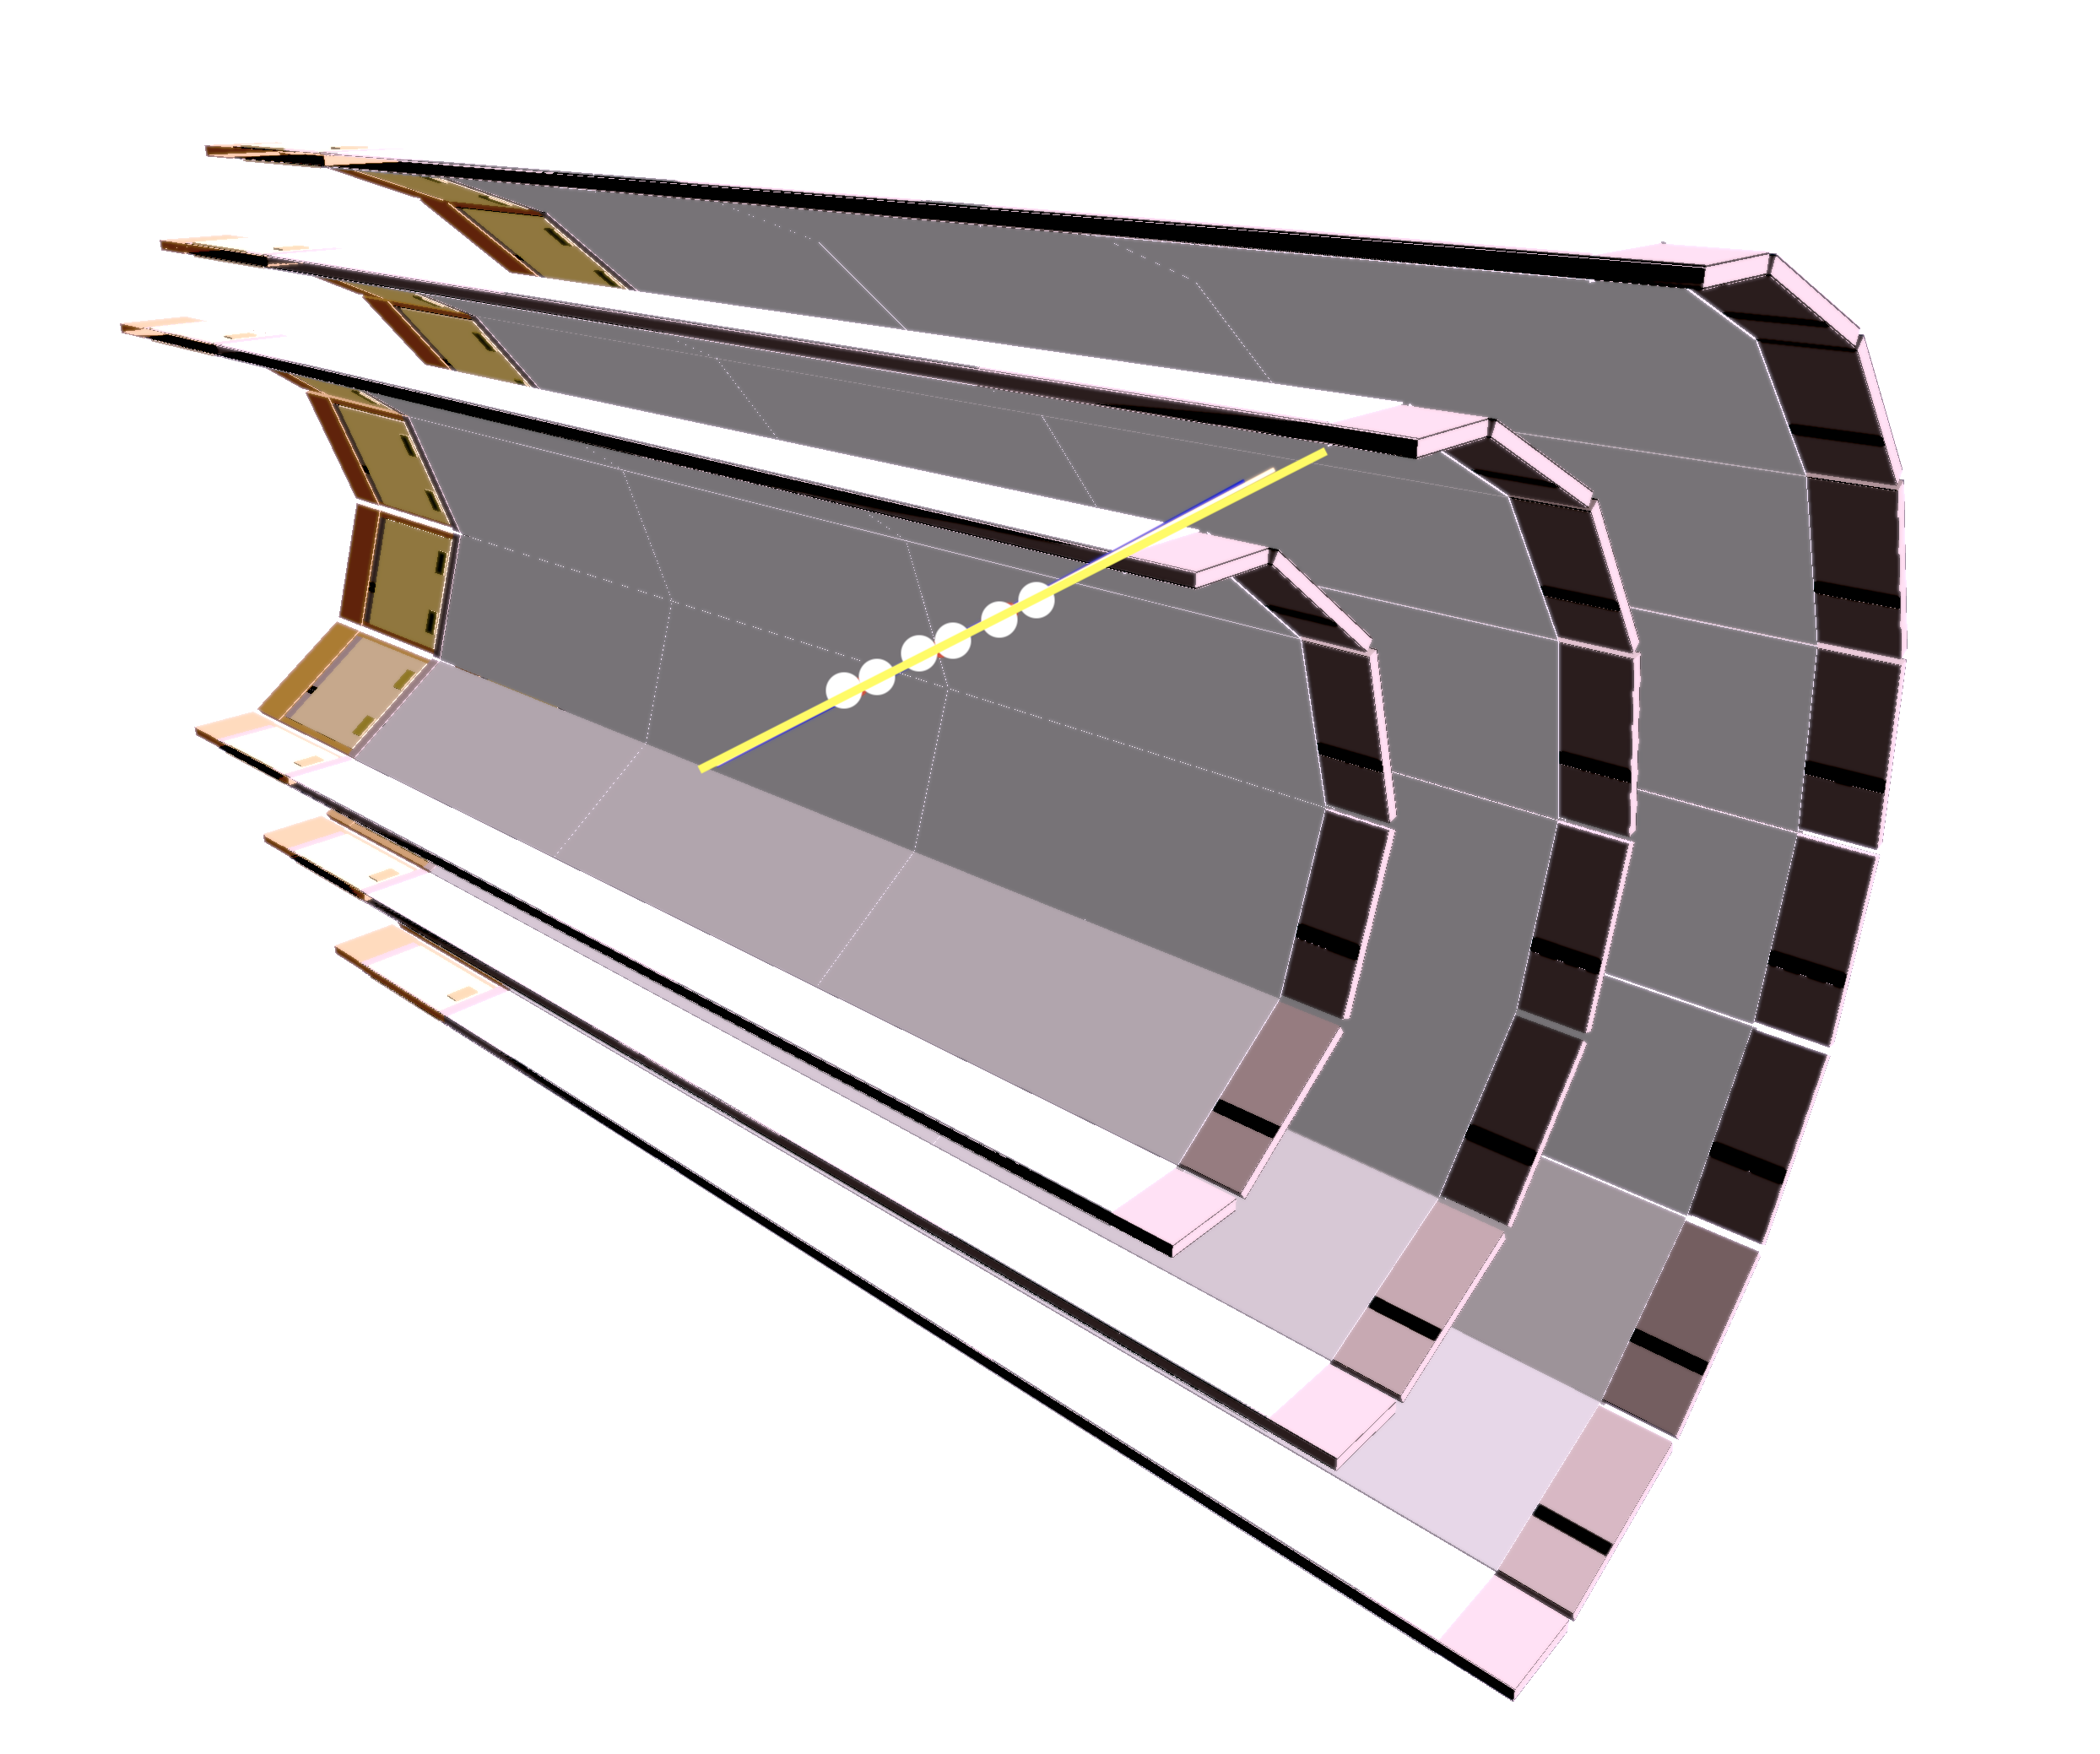
\includegraphics[width=0.99\columnwidth,keepaspectratio]{img/bstGeometry.png}
	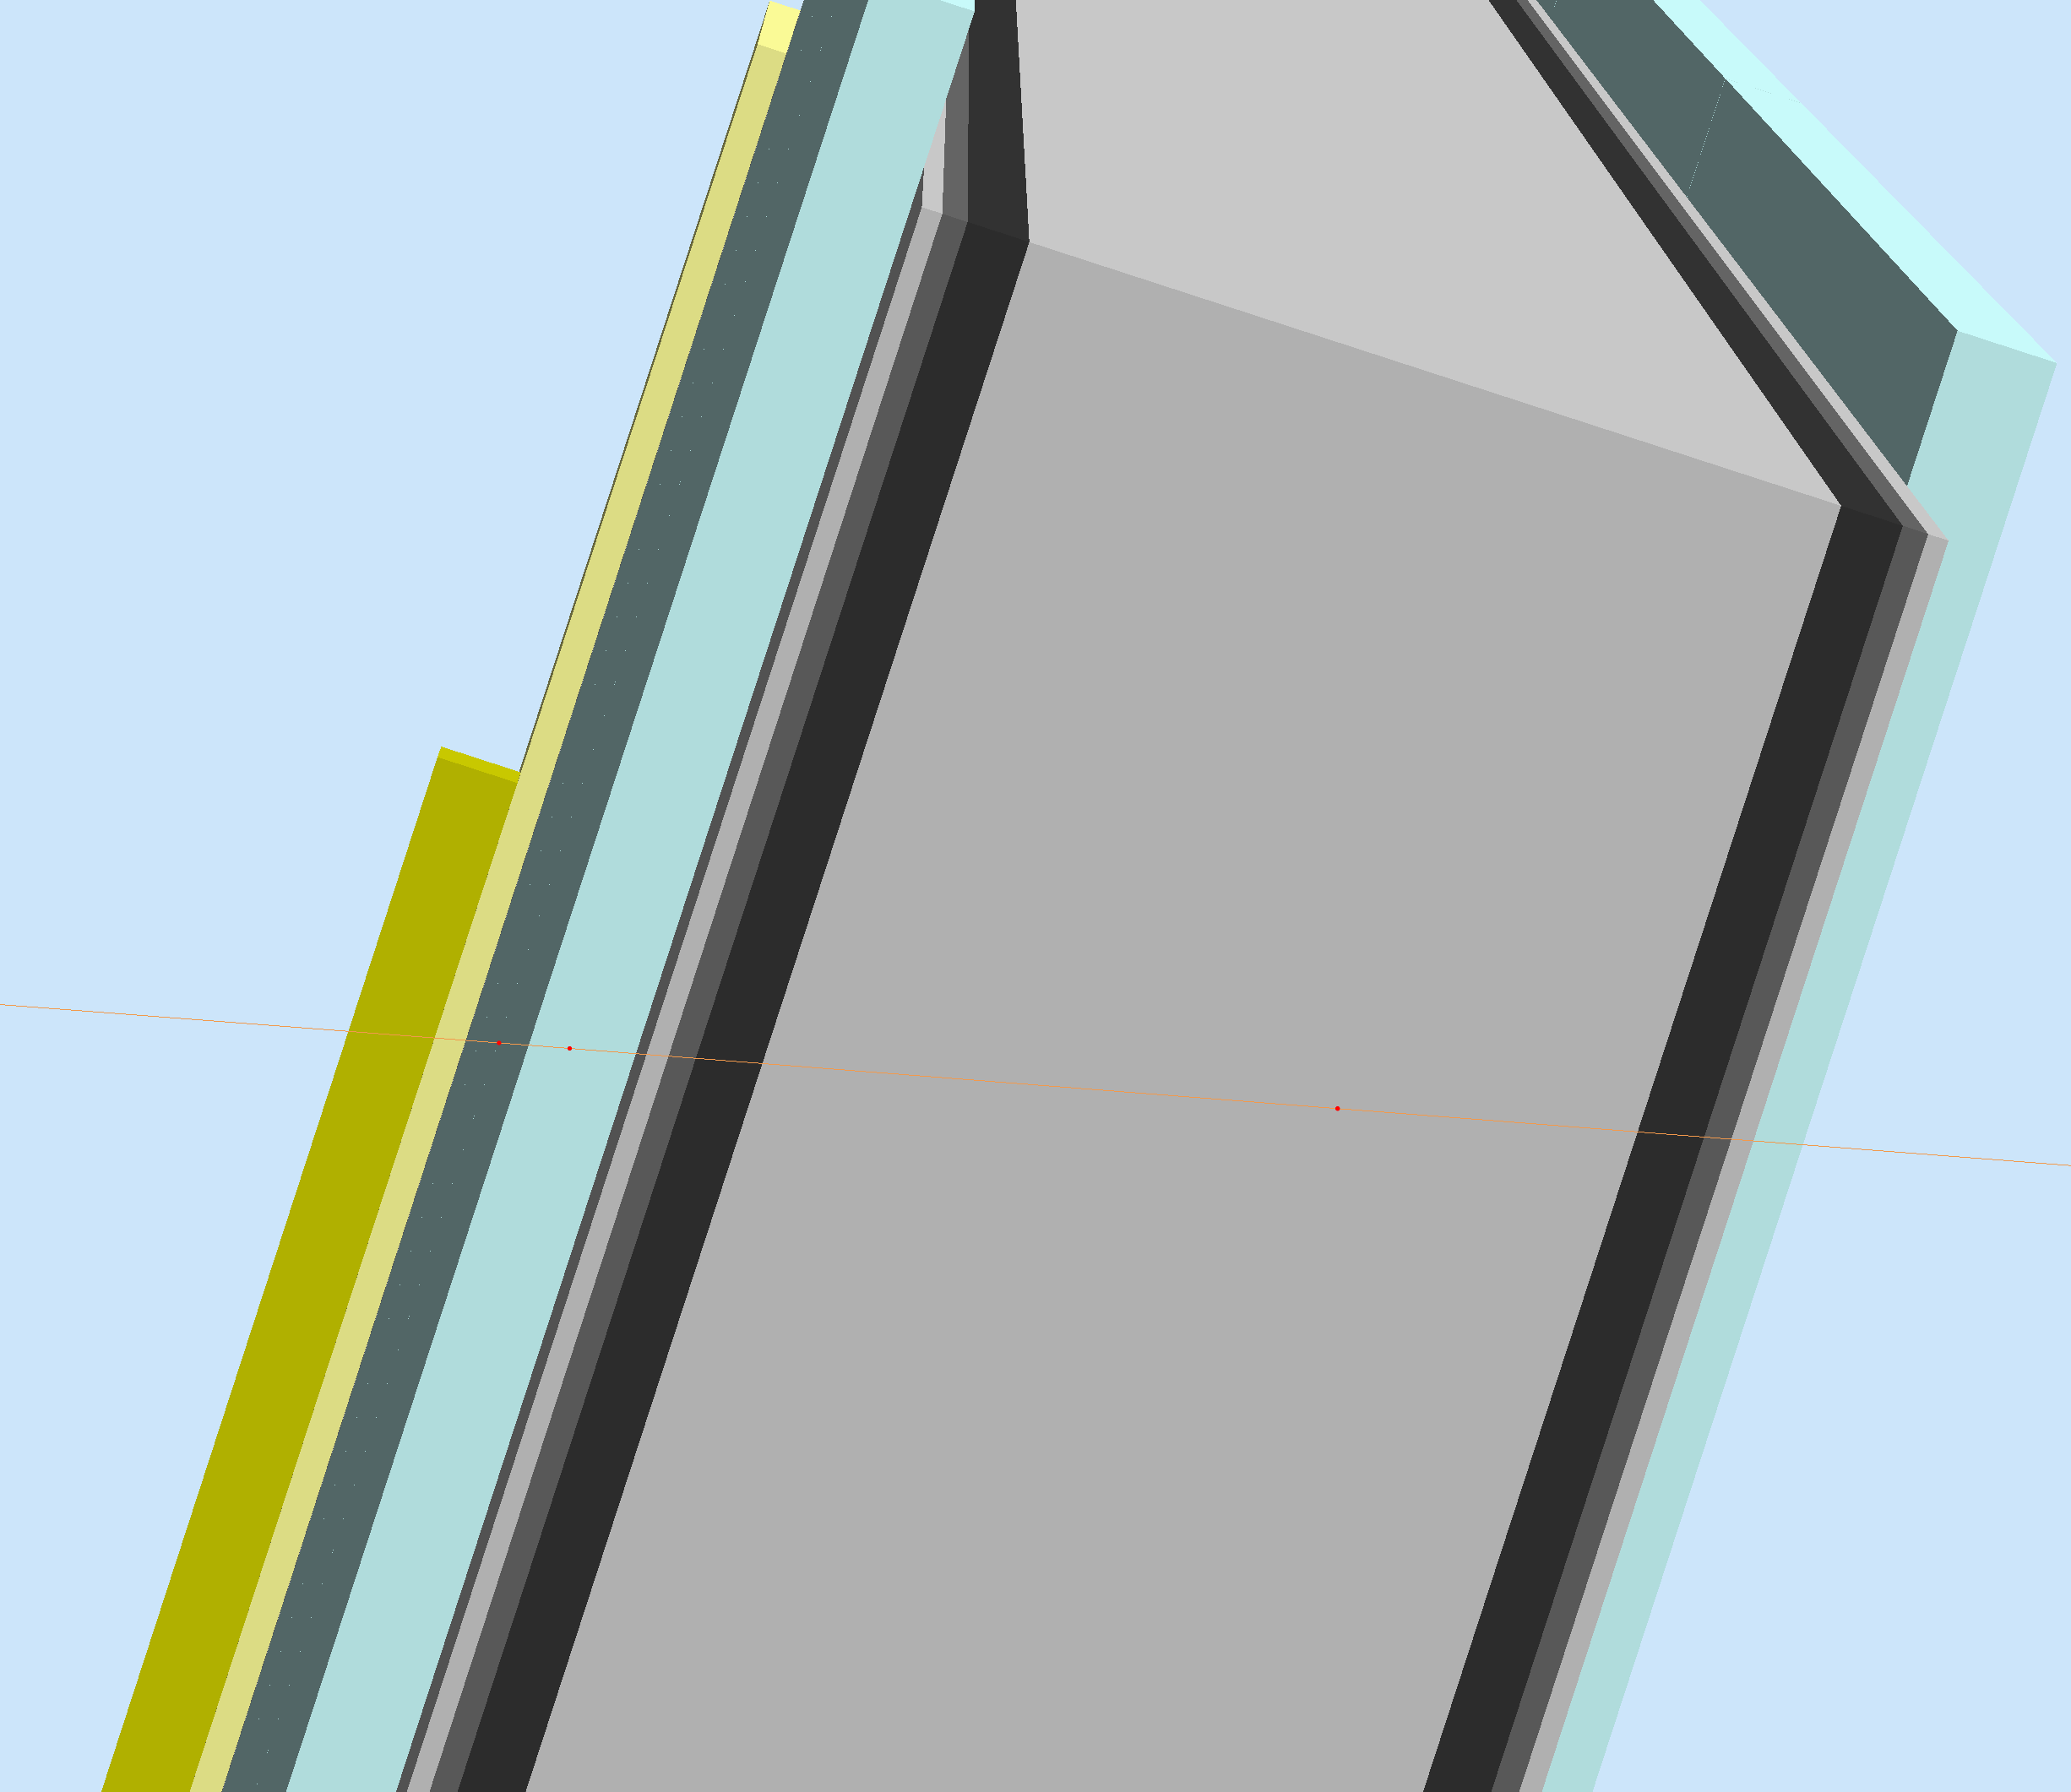
\includegraphics[width=0.99\columnwidth,keepaspectratio]{img/bstDetail.png}
	\caption{Top: the GEMC implementation of the SVT geometry. The three regions are shown in the sliced view. The silicon sensors are
           the grey color rectangles. The track is a 2 GeV proton, leaving hits (marked with white circles) in each module crossed. Bottom: detail of a module shows
           the various materials inside. The 320 $\mu$m silicon sensor is on top and bottom of the module.
           The material inside includes epoxy glue, the bus cable, and support material. The proton creates one hit
		   in both the two silicon modules it transverses.}
	\label{fig:bstGeometry}
\end{figure}


The Github location of the GEMC perl API script is at \url{https://github.com/gemc/detectors/tree/master/clas12/bst}.
The java geometry service is at
\url{https://github.com/JeffersonLab/clas12-offline-software/blob/development/common-tools/clas-jcsg/src/main/java/org/jlab/detector/geant4/v2/SVTGeant4Factory.java}


\subsubsection{Process ID}

At each Geant4 step, the local coordinates in the sensor volume are used to calculate the strip ID.
The algorithm includes: the dead zone around the sensor, the pitch between the strips (156 $\mu$m) and the angle
between the strips that varies from 0 $^{\circ}$(strip $\# 1$) to 3$^{\circ}$ (for strip  $\# 256$). A showcase of the strip ID assignment
is summarized in \F{processID}.

\begin{figure}
	\centering
	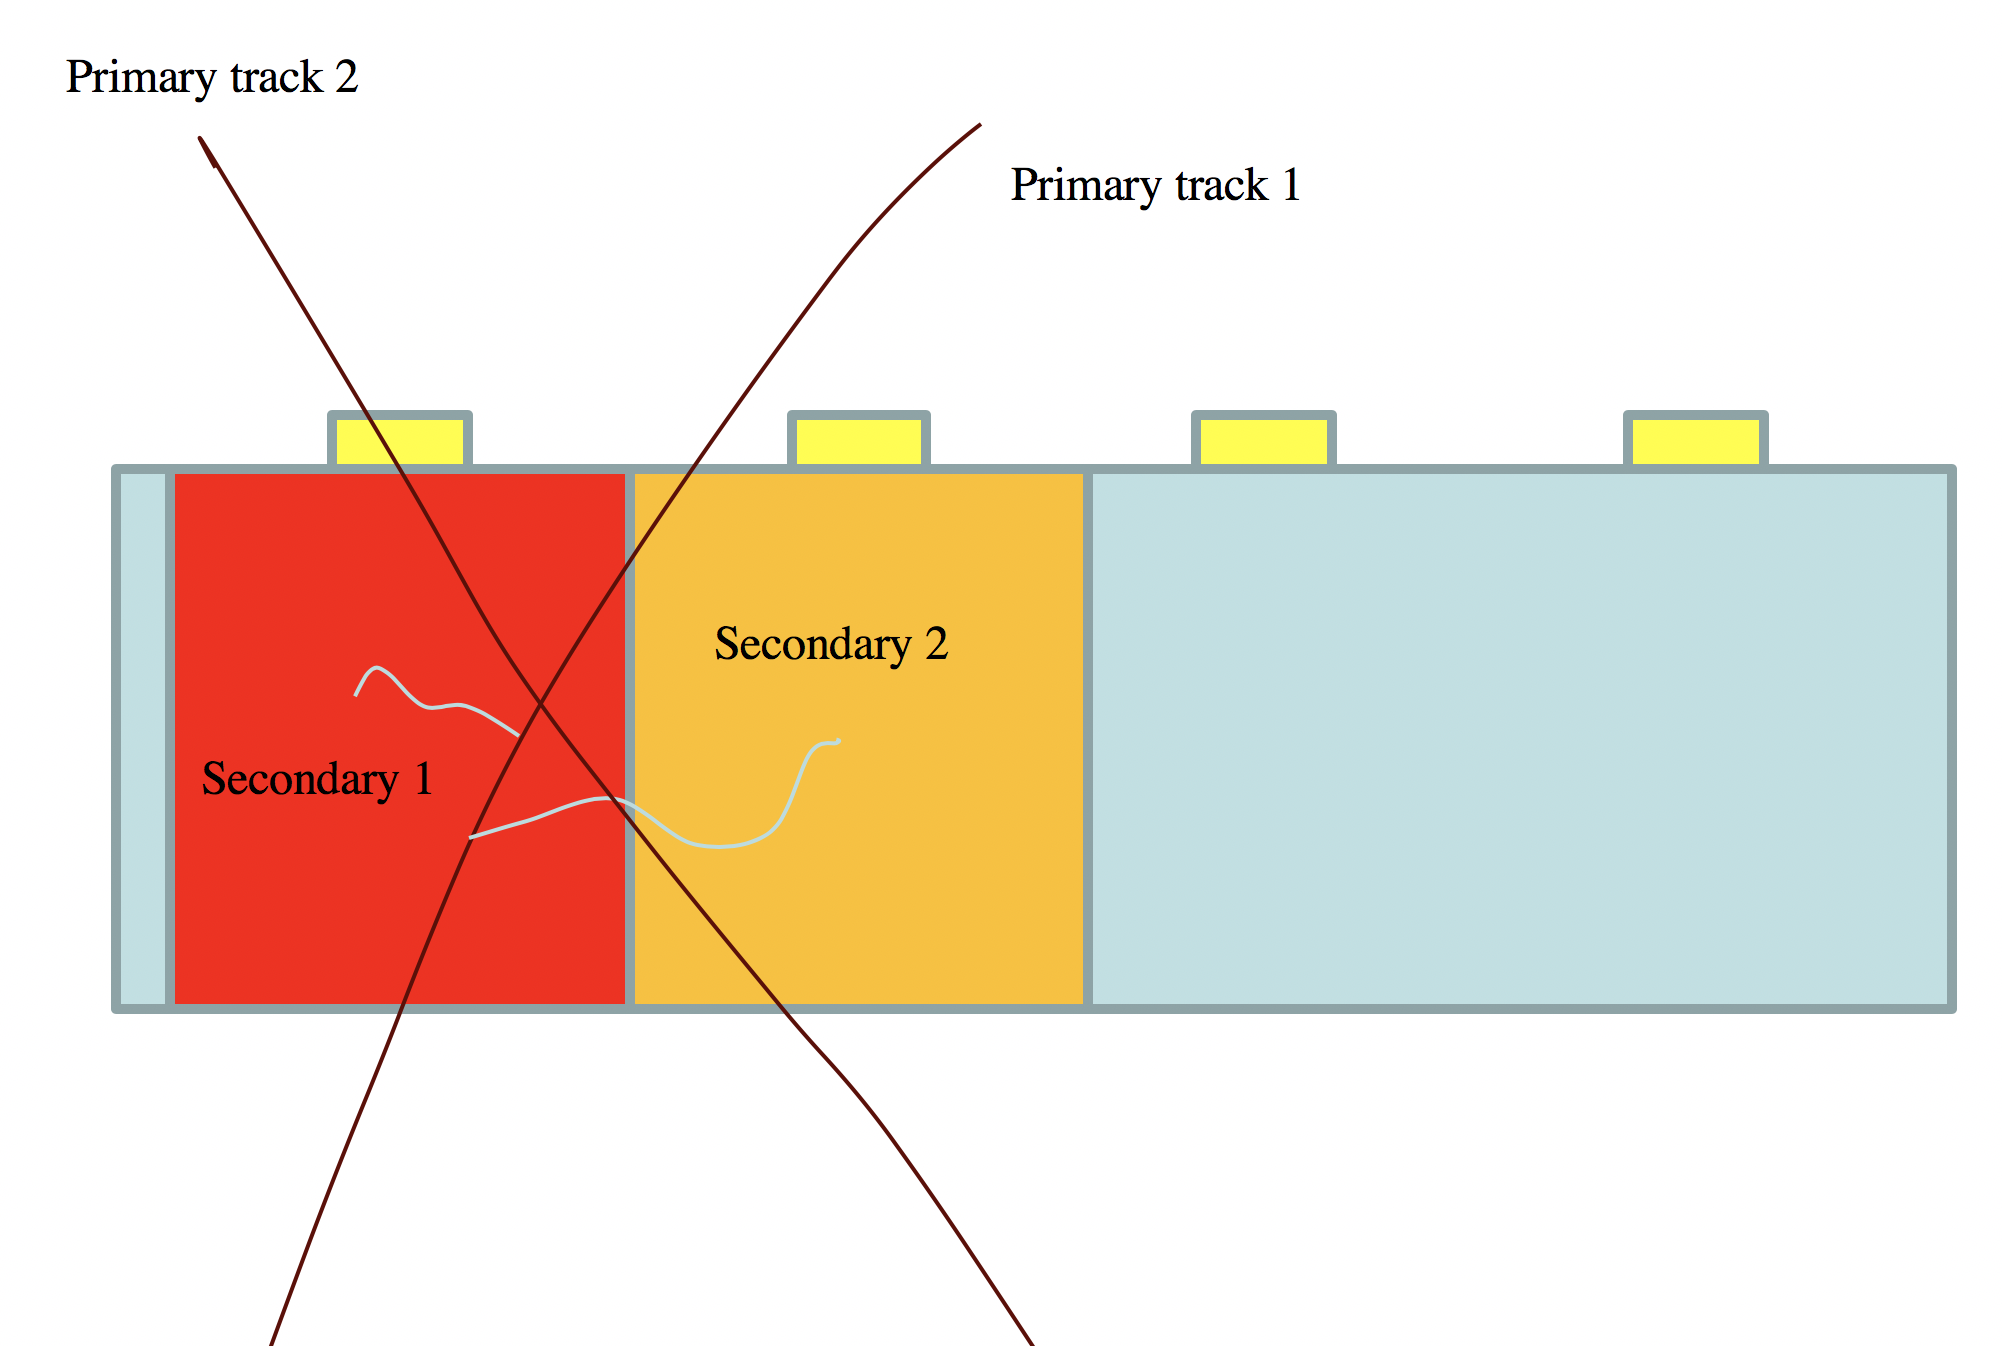
\includegraphics[width=0.99\columnwidth,keepaspectratio]{img/bstHit.png}
	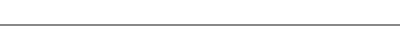
\includegraphics[width=0.99\columnwidth,keepaspectratio]{img/blank.png}
	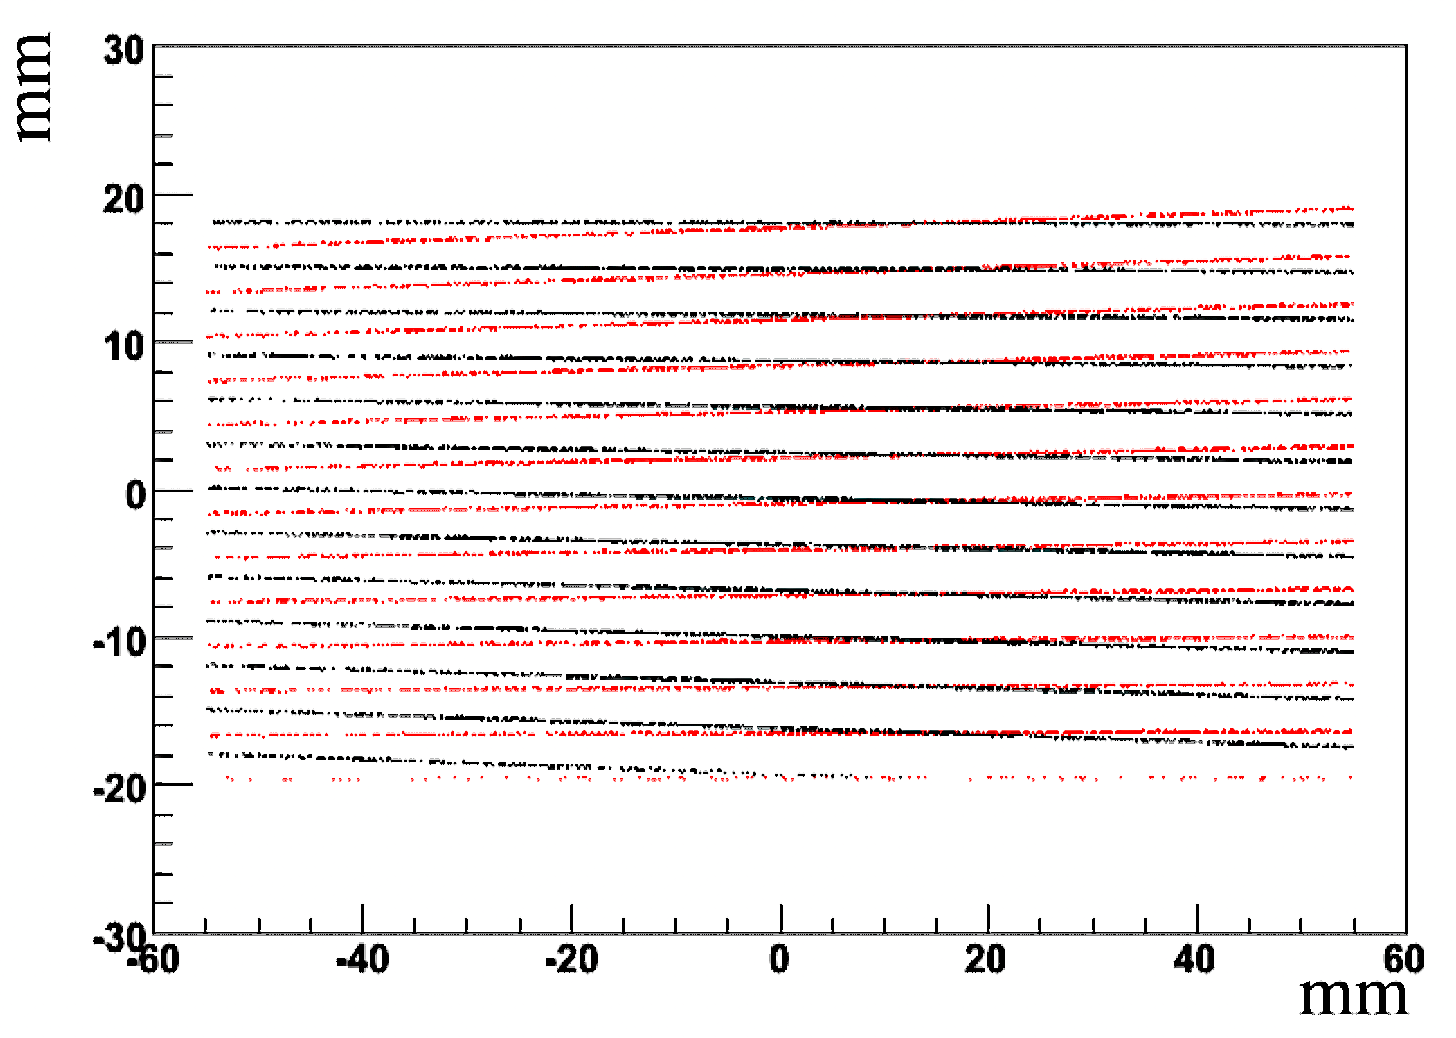
\includegraphics[width=0.99\columnwidth,keepaspectratio]{img/bstStrip.png}
	\caption{Top: process ID algorithm cartoon for SVT. The strip ID is assigned based on the local position of the track
            step within the sensitive module. If a step of the primary or the secondary particles happen between the boundary
            of the strip that was already hit, it will be assigned to that strip. Bottom: actual hit position of selected
            strips in the top and bottom silicon sensors of a module shows the fan-like distribution of the strips,
            with increasing angle. The top layer angle is opposite to the bottom layer angle. }
	\label{fig:processID}
\end{figure}

Due to the thickness of the silicon sensor, the produced electron avalanche can end up in more than one strip. This
is reproduced in the GEMC simulation using the hit sharing algorithm, see \F{bstHitSharing}.

\begin{figure}[t]
	\centering
	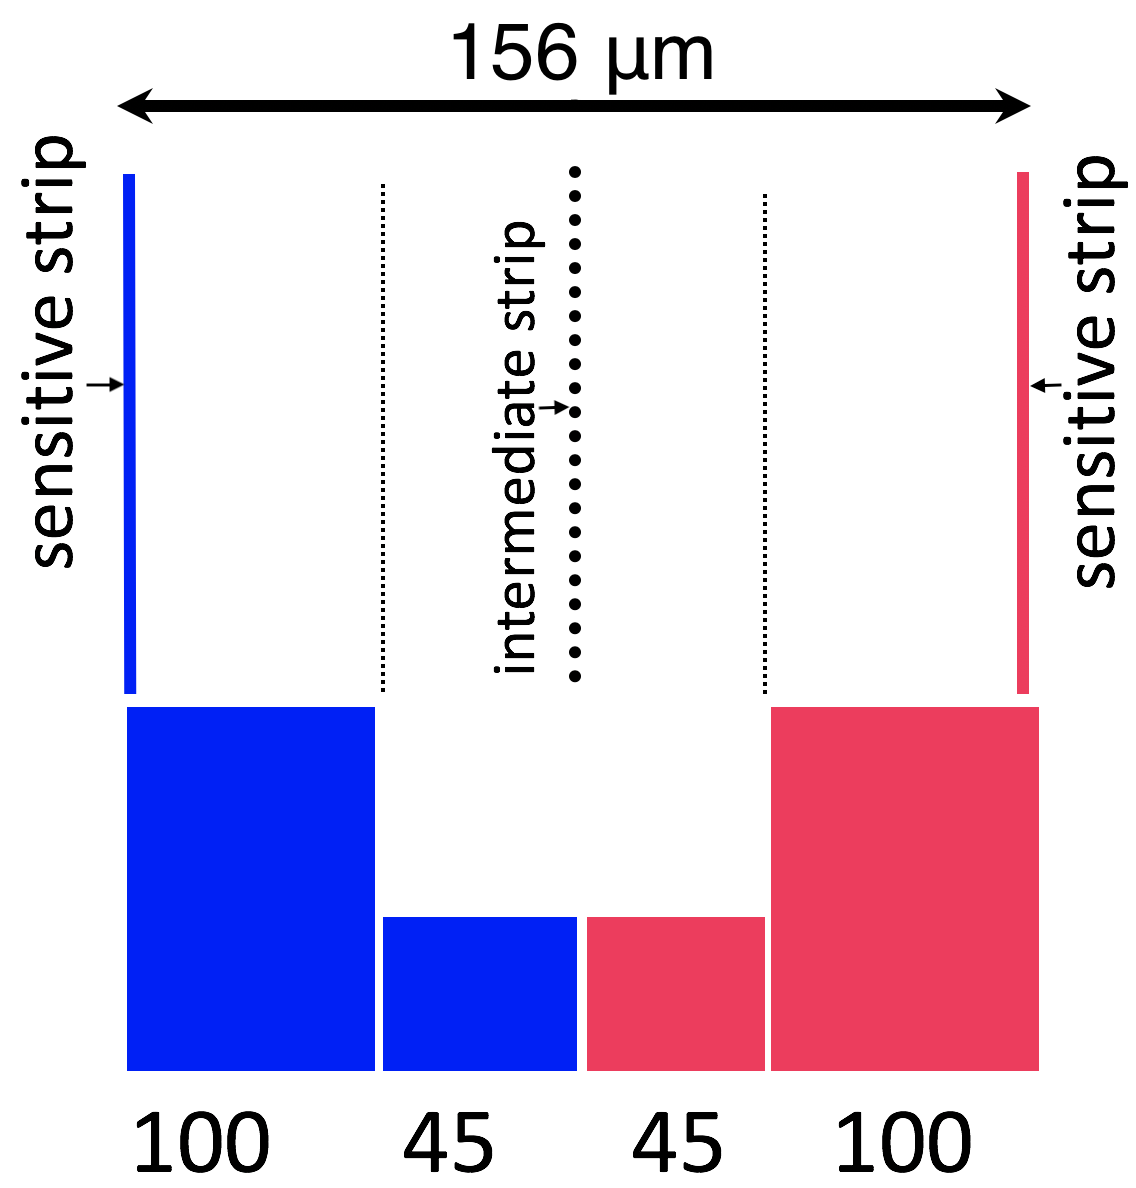
\includegraphics[width=0.99\columnwidth, height=0.65\columnwidth]{img/bstHitSharing.png}
	\caption{The SVT hit sharing algorithm. If a step in a given strip happens within 39 $\mu$m the adjacent strip, then
             $90\%$ of the energy deposited will be shared equally between them ($45\%$ each), with a $10\%$ energy loss due
	         to capacitive coupling between the strip and the backplane.}
	\label{fig:bstHitSharing}
\end{figure}


\subsubsection{Digitization}

The SVT digitization provides a 3-bit ADC, using the total energy deposited (after hit sharing) between 26 and 117 keV.
The Bunch Cross Oscillator quantity (BCO), a random number between 0 and 255,
provides the TDC timing info associated with the hit.
The digitized output bank variables are summarized in Table \ref{tab:bstBank}.

\begin{table}[h]
	\begin{center}
		\begin{tabular}{| c | c | c |}
			\hline \hline
			Variable         & Description   \\
			\hline
               layer  &                                      layer number    \\
              sector  &                                     sector number    \\
               strip  &                                      strip number    \\
                 ADC  &                                         3 bit ADC    \\
                 bco  &                                   8 bit time info    \\
               ADCHD  &                                        13 bit ADC    \\
                hitn  &                                        hit number    \\
			\hline \hline
		\end{tabular}
	\end{center}
	\caption{The digitized SVT bank.}\label{tab:bstBank}
\end{table}

\noindent The time window  of the SVT is set to to 128 ns: all geant4 steps within the same strip and time window will be collected on one hit.
The SVT hit process routines are located in the repository: \url{https://github.com/gemc/source/tree/master/hitprocess/clas12/svt}

\subsubsection{Radiation dose and background rates}
A detailed study of the background rates coming from beam interacting with the target was done to ensure that the silicon sensor
could operate in the high radiation conditions of the target proximity.

Given the nominal operating luminosity $L=10^{35}$ cm$^{-2}$s$^{-1}$, and the liquid-hydrogen target of 5 cm length, the beam electron rate
is $R=4.7 \times 10^{11} Hz$. This corresponds to about 62,000 electrons in the SVT 128 ns time window.

Simulations using 62,000 11 GeV electrons per event impinging on the liquid-hydrogen target were analyzed.
The rates were calculated for the various Regions and for different thresholds, see \F{radStudyThreshold}.


\begin{figure}
	\centering
	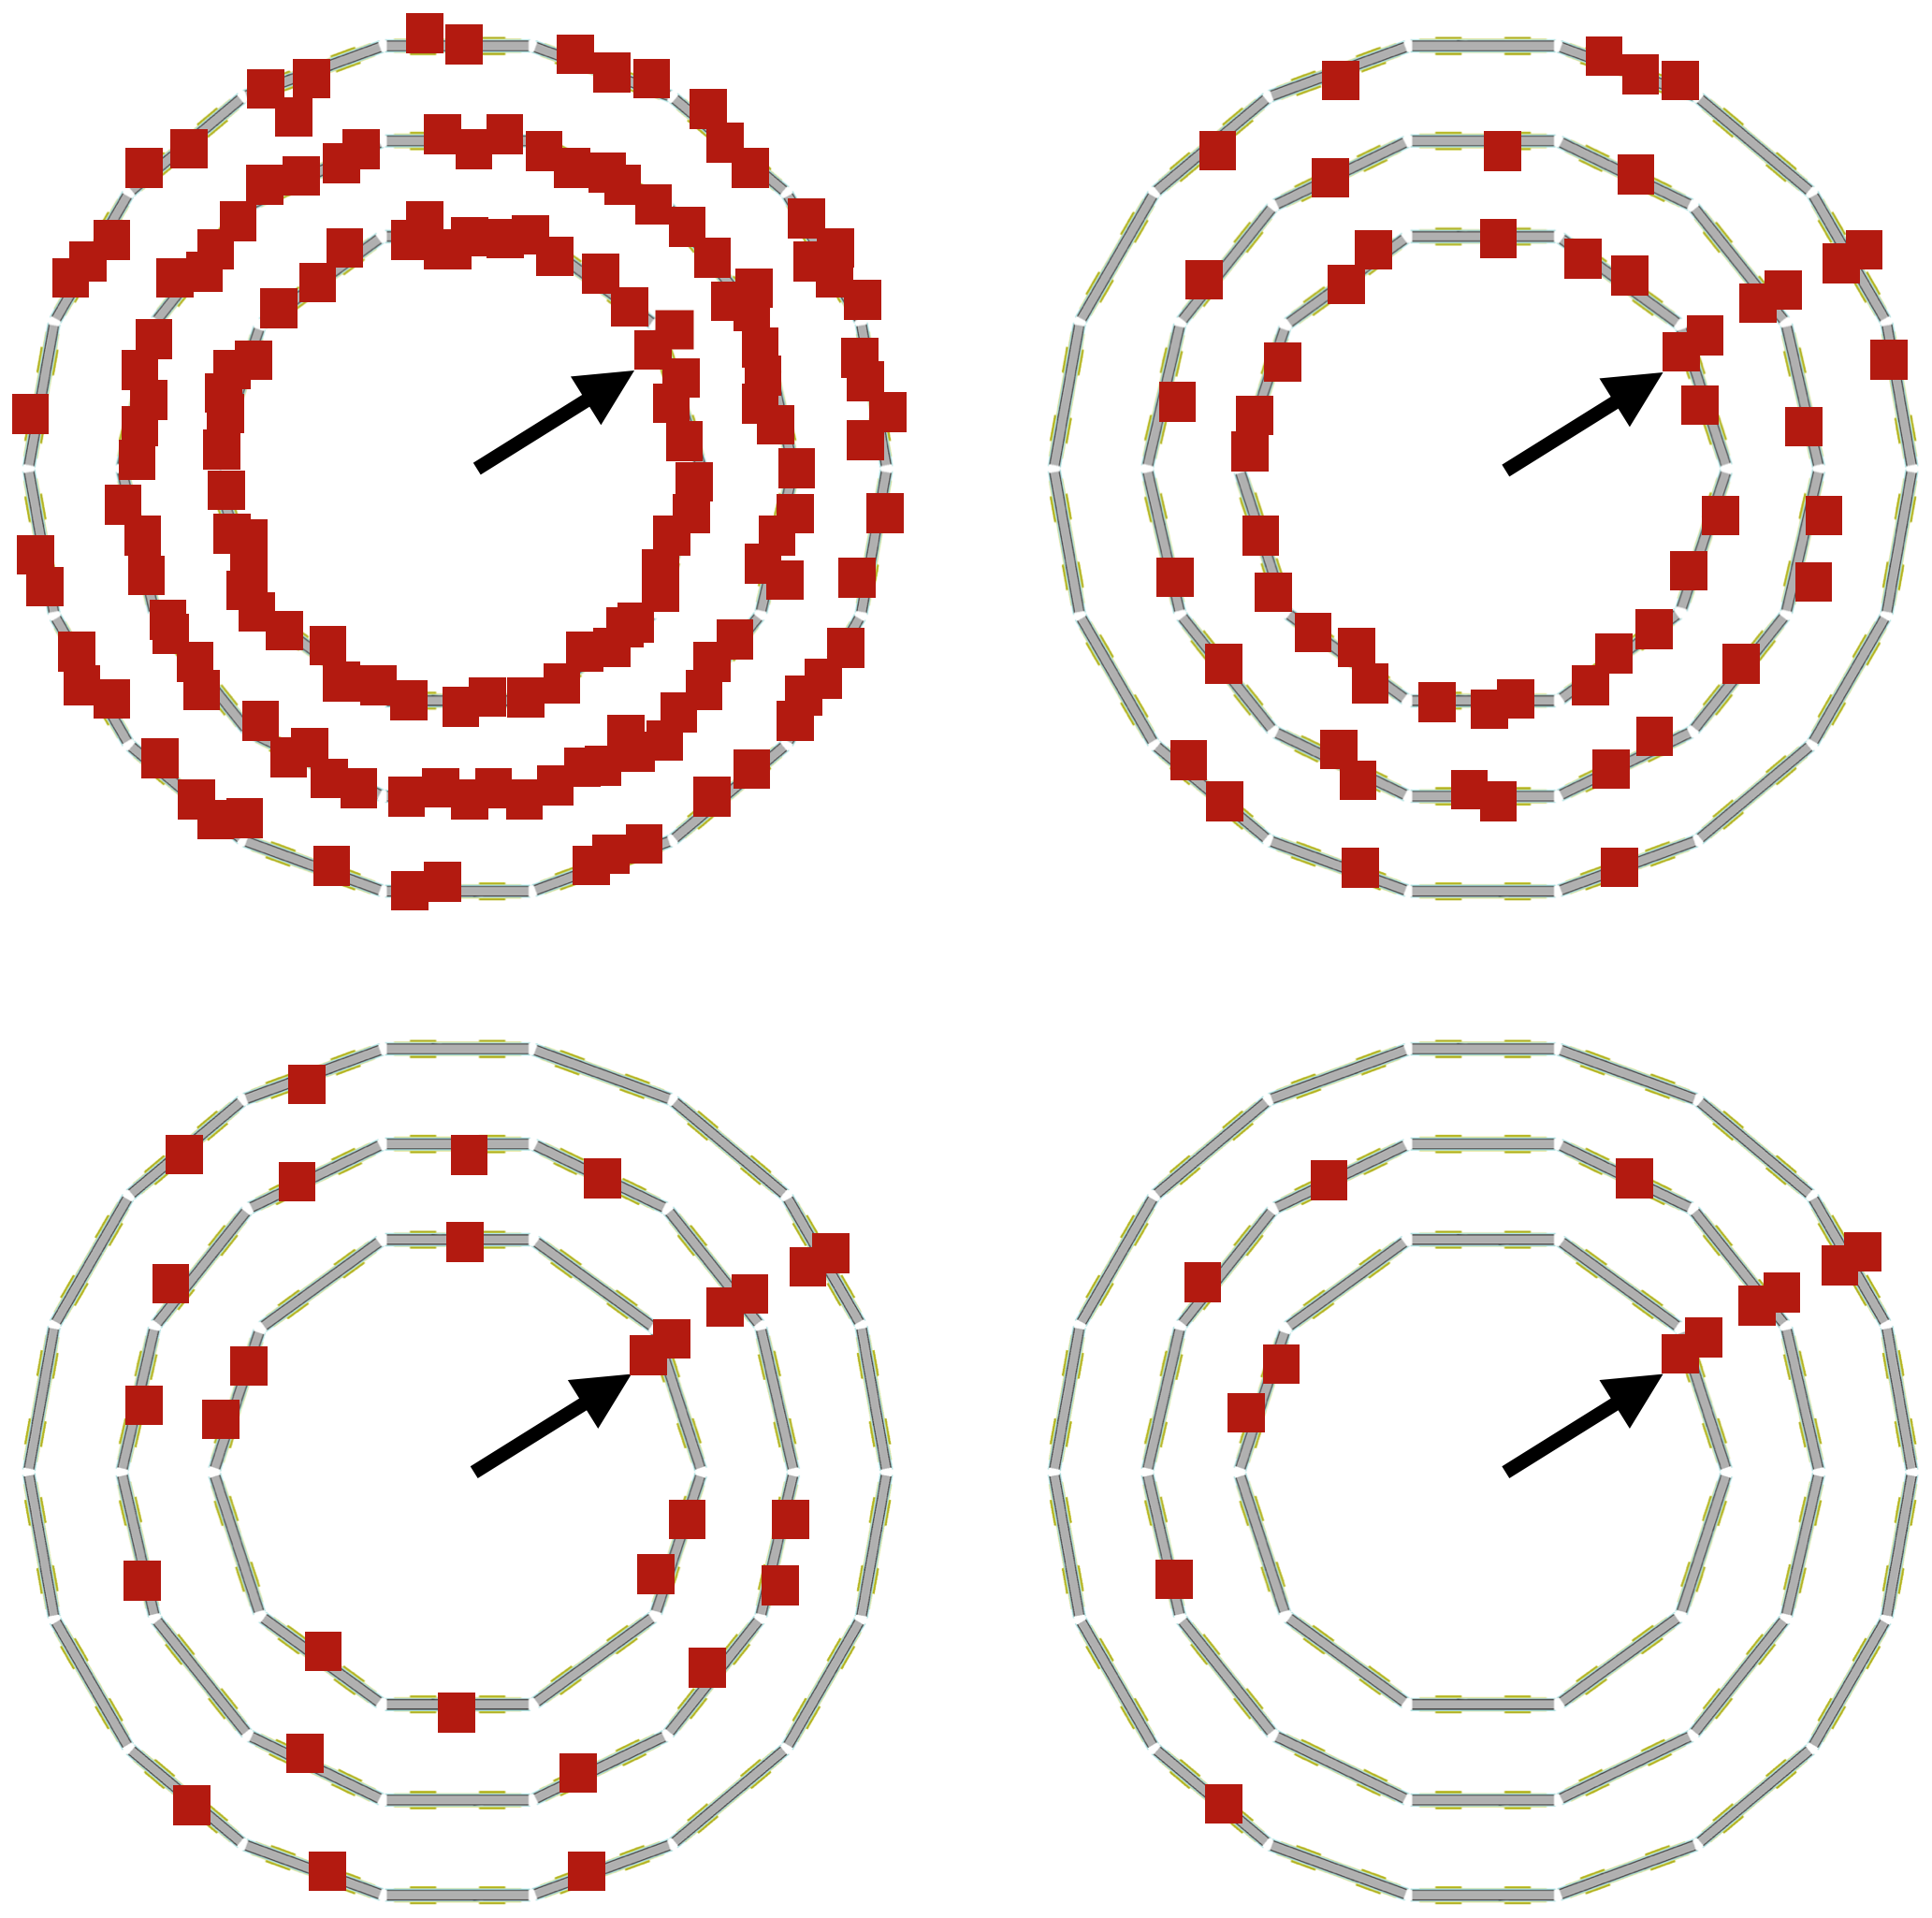
\includegraphics[width=0.99\columnwidth,keepaspectratio]{img/bstHitDisplay.png}
	\caption{The occupancy in the various SVT layers for different thresholds for one event containing a proton track (direction indicated
             by the arrow). The hits are represented by the circles.
             Top left: with no energy cut, all SVT layers are hit wih numerous hits. Many are photons leaving no energy, as shown in
             bottom left where the condition of some energy deposition is required. Top right: 20 KeV energy threshold. Bottom right:
             with 40 KeV energy threshold, the proton track hits survive and only a handful of background hits are visible.}
	\label{fig:radStudyThreshold}
\end{figure}


The radiation dose and the 1 MeV neutron equivalent damage was estimated. Most of the radiation
is released in the first two layers of the SVT.
The 370 rad / year are low enough to grant the SVT operation for 15 years. The results of the study
are summarized in \F{radStudy}.


\begin{figure}
	\centering
	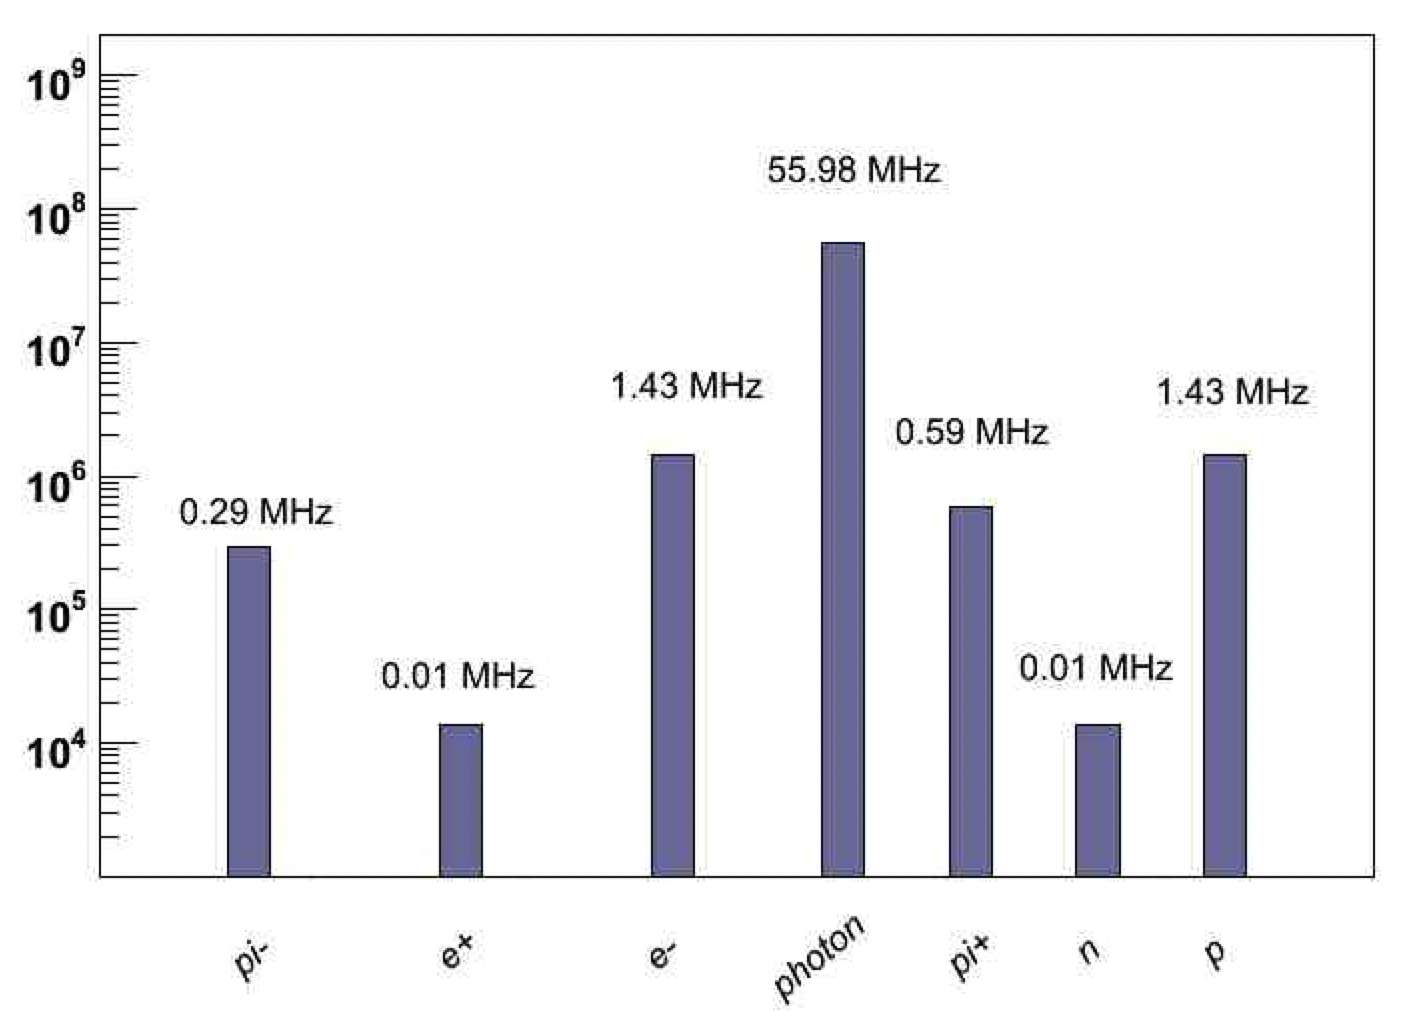
\includegraphics[width=0.99\columnwidth,keepaspectratio]{img/bstRates.png}
	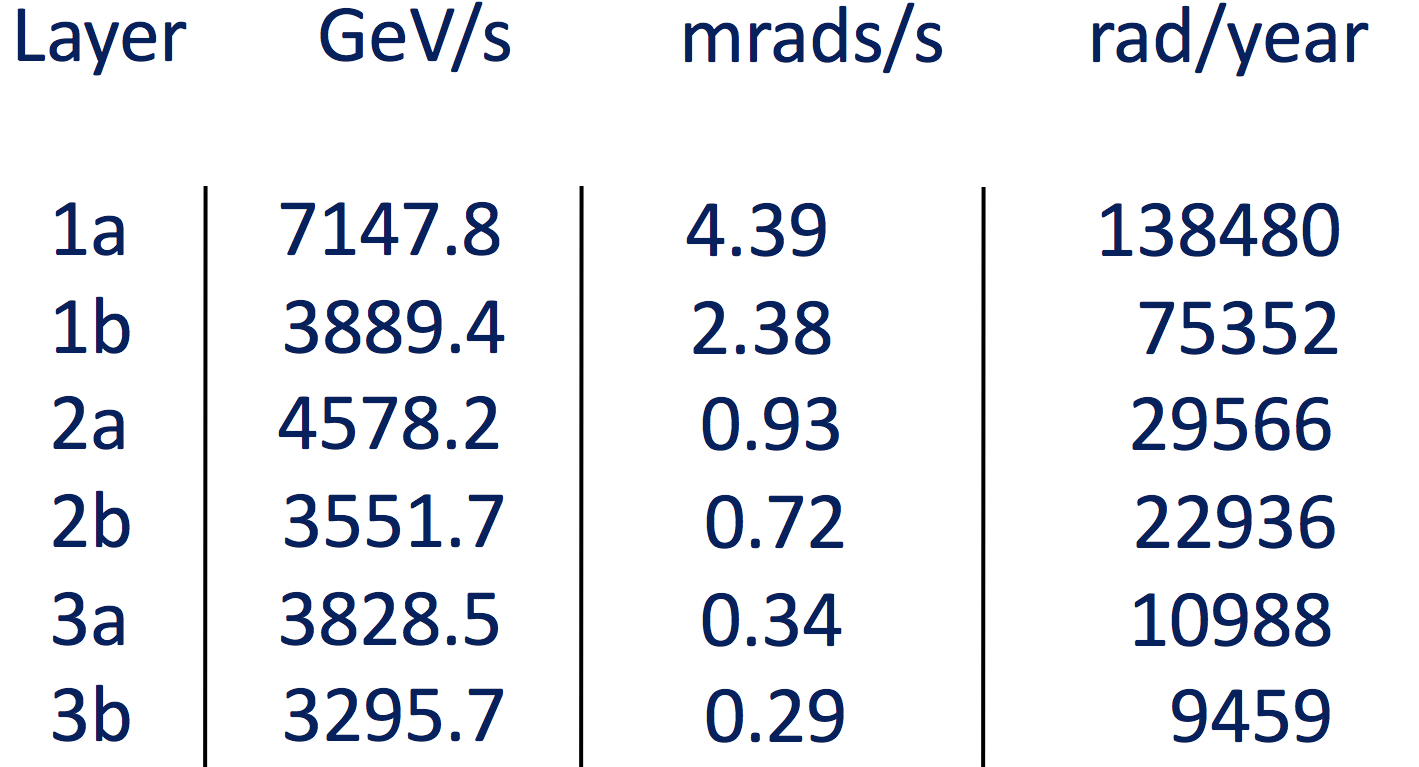
\includegraphics[width=0.99\columnwidth,keepaspectratio]{img/bstRadSummary.png}
	\caption{Summary of radiation doses and background rates in the SVT. Top: the rate breakdown for different particles
             for a threshold of 20 keV (the current hardware threshold is 30 keV) at the full luminosity of CLAS12.
             Bottom: table showing the fluences and radiation doses in the SVT layers. }
	\label{fig:radStudy}
\end{figure}

In addition a thin layer of tungsten (51 $\mu$m) was added between the target and the inner SVT layer aimed at reducing the electromagnetic
background \cite{bstDose}.





